\documentclass[border=10pt]{standalone}
\usepackage[svgnames]{xcolor}
\usepackage{amsmath}
\usepackage{pgfplots}
\pgfplotsset{compat=newest}
\usepackage[sfdefault]{FiraSans}
\usepackage{FiraMono}
\renewcommand*\familydefault{\sfdefault}
\begin{document}
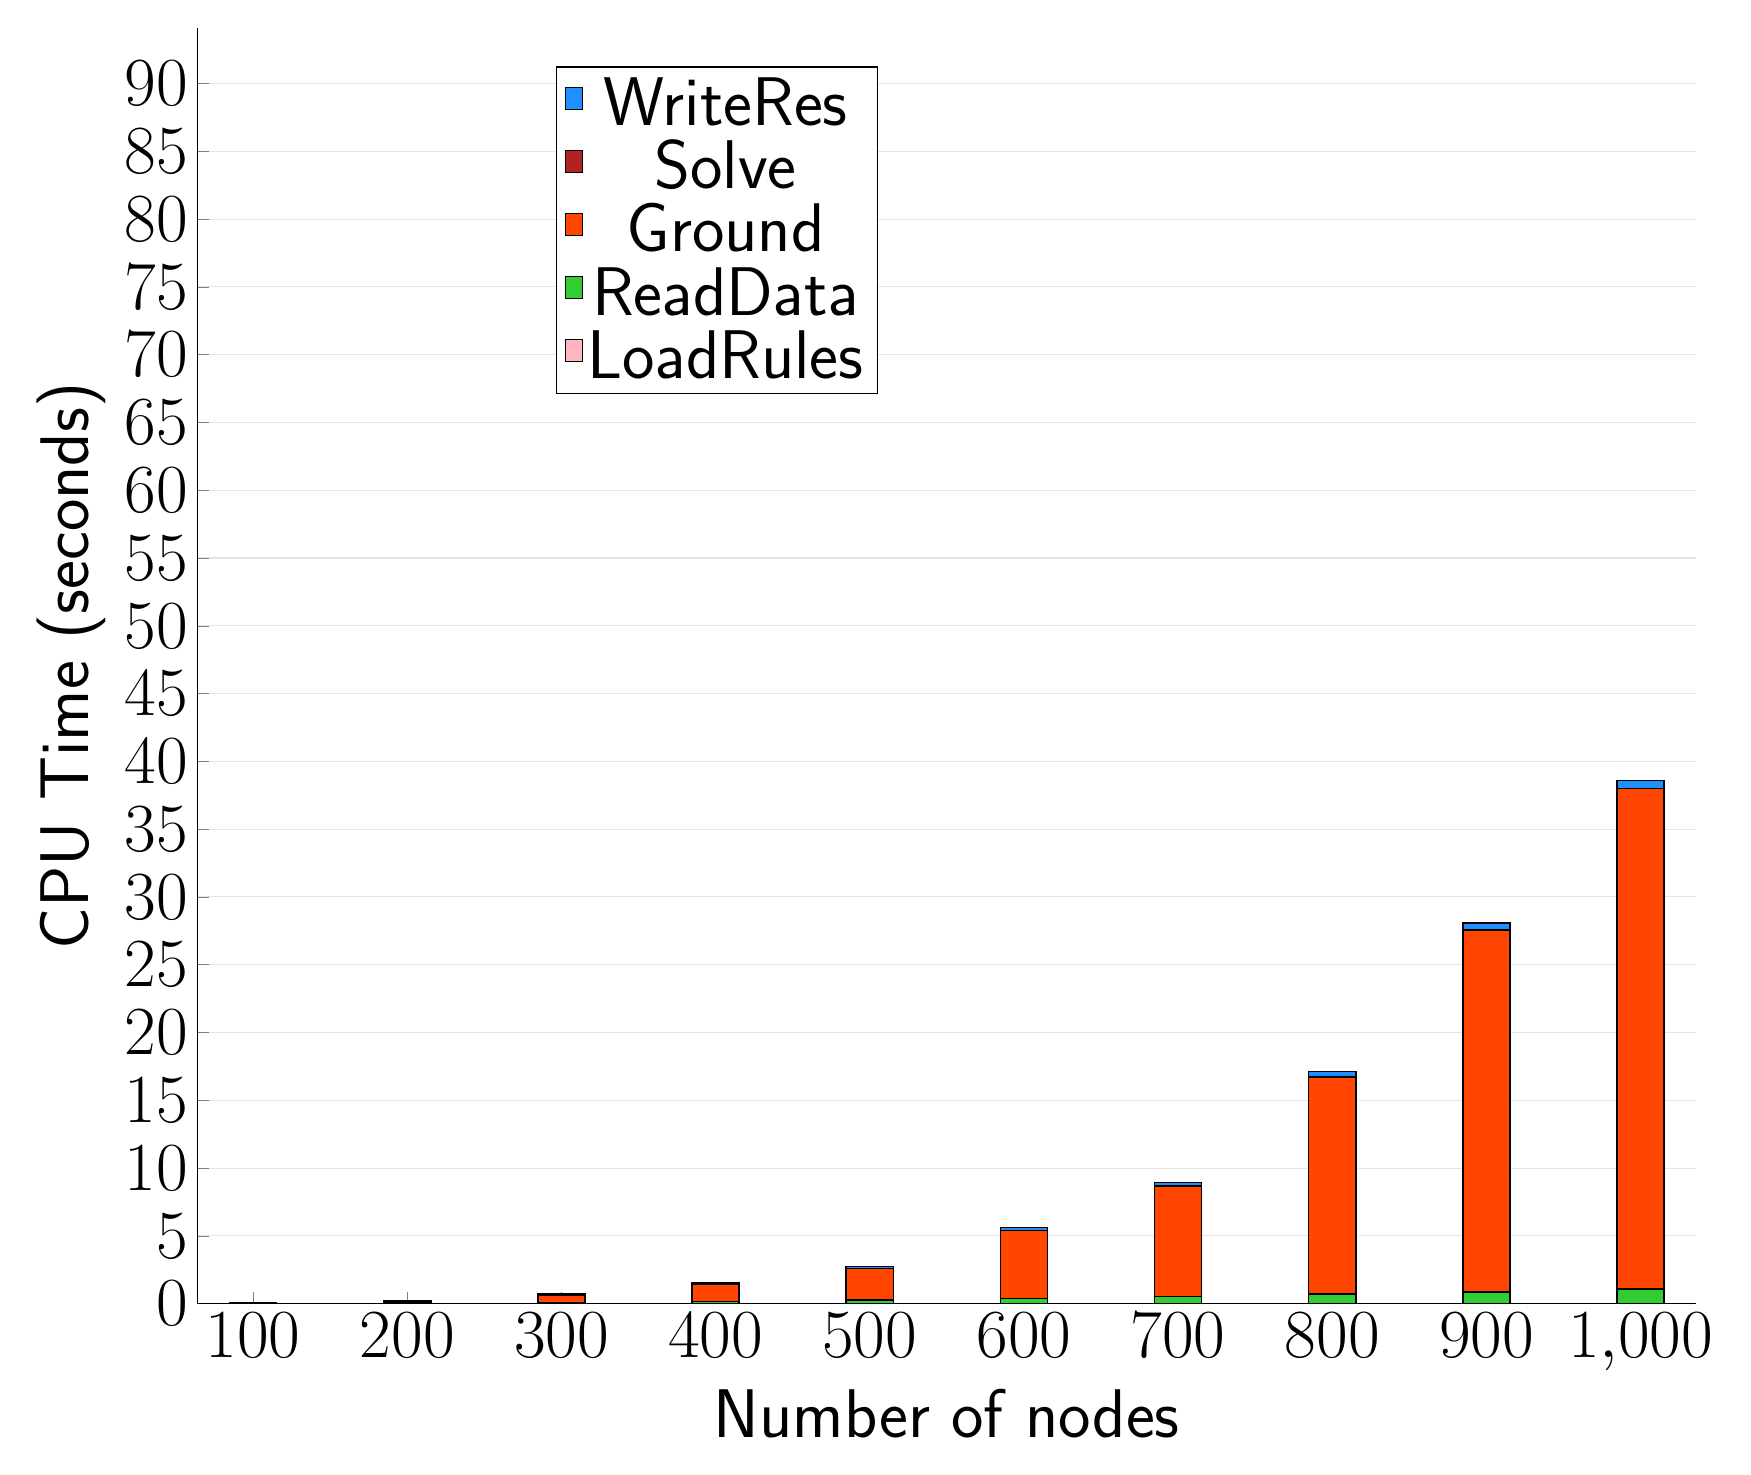
\begin{tikzpicture}
\begin{axis}[
   ybar stacked,
   width=1.7\textwidth,
   bar width=0.6cm,
   ymajorgrids, tick align=inside,
   major grid style={draw=gray!20},
   xtick=data,
   ymin=0, ymax=94.08204,
   axis x line*=bottom,
   axis y line*=left,
   enlarge x limits=0.04,
   legend style={
       at={(0.454, 0.97)},
       anchor=north east,
       legend columns=1,
       font=\Huge,
   },
   ylabel={CPU Time (seconds)},
   xlabel={Number of nodes},
   label style={font=\Huge},
   tick label style={font=\Huge},
]
\addlegendimage{fill=DodgerBlue, draw=black, line width=0.2pt}
\addlegendentry{WriteRes}
\addlegendimage{fill=FireBrick, draw=black, line width=0.2pt}
\addlegendentry{Solve}
\addlegendimage{fill=OrangeRed, draw=black, line width=0.2pt}
\addlegendentry{Ground}
\addlegendimage{fill=LimeGreen, draw=black, line width=0.2pt}
\addlegendentry{ReadData}
\addlegendimage{fill=LightPink, draw=black, line width=0.2pt}
\addlegendentry{LoadRules}
\addplot +[fill=LightPink, draw=black, line width=0.55pt] coordinates {
(100, 0.0)
(200, 0.0)
(300, 0.0)
(400, 0.0)
(500, 0.0)
(600, 0.0)
(700, 0.0)
(800, 0.0)
(900, 0.0)
(1000, 0.0)
};
\addplot +[fill=LimeGreen, draw=black, line width=0.55pt] coordinates {
(100, 0.010000000000000009)
(200, 0.040000000000000036)
(300, 0.09200000000000003)
(400, 0.16999999999999998)
(500, 0.268)
(600, 0.38599999999999995)
(700, 0.5360000000000001)
(800, 0.7040000000000001)
(900, 0.874)
(1000, 1.0879999999999999)
};
\addplot +[fill=OrangeRed, draw=black, line width=0.55pt] coordinates {
(100, 0.020000000000000018)
(200, 0.15799999999999997)
(300, 0.554)
(400, 1.252)
(500, 2.332)
(600, 5.008)
(700, 8.108)
(800, 16.028000000000002)
(900, 26.682)
(1000, 36.894000000000005)
};
\addplot +[fill=FireBrick, draw=black, line width=0.55pt] coordinates {
(100, 0.0)
(200, 0.0020000000000000018)
(300, 0.0020000000000000018)
(400, 0.0040000000000000036)
(500, 0.007999999999999919)
(600, 0.010000000000000142)
(700, 0.013999999999999702)
(800, 0.021999999999999176)
(900, 0.0260000000000002)
(1000, 0.03400000000000074)
};
\addplot +[fill=DodgerBlue, draw=black, line width=0.55pt] coordinates {
(100, 0.010000000000000009)
(200, 0.018000000000000016)
(300, 0.05199999999999998)
(400, 0.09600000000000009)
(500, 0.14400000000000013)
(600, 0.20999999999999983)
(700, 0.28800000000000037)
(800, 0.35800000000000093)
(900, 0.4759999999999994)
(1000, 0.5819999999999992)
};
\end{axis}
\end{tikzpicture}

\end{document}
